\documentclass[10pt, a4paper, landscape]{article}

% ----- packages -----
\usepackage{amsmath} % AMS mathematical facilities for LaTeX
\usepackage{amssymb}
\usepackage{enumitem} % Control layout of itemize, enumerate, description
\usepackage{fancyhdr} % Extensive control of page headers and footers in LaTeX2
\usepackage{geometry} % Flexible and complete interface to document dimensions
\usepackage{graphicx} % Enhanced support for graphics
\usepackage{hyperref} % Extensive support for hypertext in LaTeX
\usepackage{multicol} % Intermix single and multiple columns
\usepackage{parskip} % Layout with zero \parindent, non-zero \parskip
\usepackage{tikz} % Create PostScript and PDF graphics in TeX
\usepackage{titlesec} % Select alternative section titles

% ----- random seed -----
\pgfmathsetseed{10}

% ----- custom commands -----
\newcommand{\E}{\mathrm{E}}
\newcommand{\Var}{\mathrm{Var}}
\newcommand{\se}{\mathrm{se}}
\newcommand{\Cov}{\mathrm{Cov}}
\newcommand{\Corr}{\mathrm{Corr}}
\newcommand{\SSR}{\mathrm{SSR}}
\newcommand{\SSE}{\mathrm{SSE}}
\newcommand{\SST}{\mathrm{SST}}
\newcommand{\tr}{\mathsf{T}}
\newcommand{\rk}{\mathrm{rk}}

% ----- page customization -----
\geometry{margin=1cm} % margins config
\pagenumbering{gobble} % remove page numeration
\setlength{\parskip}{0cm} % paragraph spacing
% title spacing
\titlespacing{\section}{0pt}{2ex}{1ex}
\titlespacing{\subsection}{0pt}{1ex}{0ex}
\titlespacing{\subsubsection}{0pt}{0.5ex}{0ex}

% ----- footer -----
\pagestyle{fancy}
\renewcommand{\headrulewidth}{0pt}
\cfoot{\href{https://github.com/marcelomijas/econometrics-cheatsheet}{\normalfont \footnotesize ADD-25.01-EN - github.com/marcelomijas/econometrics-cheatsheet - CC-BY-4.0 license}}
\setlength{\footskip}{12pt}

% ----- document -----
\begin{document}
	\begin{multicols}{3}
		\begin{center}
			\textbf{\LARGE \href{https://github.com/marcelomijas/econometrics-cheatsheet}{Additional Cheat Sheet}}
			
			{\footnotesize By Marcelo Moreno - Universidad Rey Juan Carlos}
			
			{\footnotesize The Econometrics Cheat Sheet Project}
		\end{center}
		
		\section*{OLS matrix notation}
		
		The general econometric model:
		
		\begin{center}
			$y_{i} = \beta_{0} + \beta_{1} x_{1i} + \cdots + \beta_{k} x_{ki} + u_{i}$
		\end{center}
		
		Can be written in matrix notation as:
		
		\begin{center}
			$y = X \beta + u$
		\end{center}
		
		Let's call $\hat{u}$ the vector of estimated residuals ($\hat{u} \neq u$):
		
		\begin{center}
			$\hat{u} = y - X \hat{\beta}$
		\end{center}
		
		The \textbf{objective} of OLS is to \textbf{minimize} the SSR:
		
		\begin{center}
			$\min \SSR = \min \sum_{i=1}^{n} \hat{u}_{i}^{2} = \min \hat{u}^{\tr} \hat{u}$
		\end{center}
		
		\begin{itemize}[leftmargin=*]
			\item Defining $\hat{u}^{\tr} \hat{u}$:
			
			\begin{center}
				$\hat{u}^{\tr} \hat{u} = (y - X \hat{\beta})^{\tr} (y - X \hat{\beta}) =$
				
				$= y^{\tr} y - 2 \hat{\beta}^{\tr} X^{\tr} y + \hat{\beta}^{\tr} X^{\tr} X \hat{\beta}$
			\end{center}
			
			\item Minimizing $\hat{u}^{\tr} \hat{u}$:
			
			\begin{center}
				$\frac{\partial \hat{u}^{\tr} \hat{u}}{\partial \hat{\beta}} = -2 X^{\tr} y + 2 X^{\tr} X \hat{\beta} = 0$
				
				$\hat{\beta} = (X^{\tr} X)^{-1} (X^{\tr} y)$
				
				\scalebox{0.85}{
					$
					\begin{bmatrix}
						\beta_{0} \\
						\beta_{1} \\
						\vdots    \\
						\beta_{k}
					\end{bmatrix}
					=
					\begin{bmatrix}
						n          & \sum x_{1}       & \hdots & \sum x_{k}       \\
						\sum x_{1} & \sum x_{1}^{2}   & \hdots & \sum x_{1} x_{k} \\
						\vdots     & \vdots           & \ddots & \vdots           \\
						\sum x_{k} & \sum x_{k} x_{1} & \hdots & \sum x_{k}^{2}
					\end{bmatrix}^{-1}\cdot
					\begin{bmatrix}
						\sum y       \\
						\sum y x_{1} \\
						\vdots       \\
						\sum y x_{k}
					\end{bmatrix}
					$ 
				}
			\end{center}
			
			The second derivative $\frac{\partial^{2} \hat{u}^{\tr} \hat{u}}{\partial \hat{\beta}^{2}} = X^{\tr} X > 0$ (is a min.)
		\end{itemize}
		
		\section*{Variance-covariance matrix of $\hat{\beta}$}
		
		Has the following shape:
		
		\begin{center}
			$\Var(\hat{\beta}) = \hat{\sigma}^{2}_{u} \cdot (X^{\tr} X)^{-1}=$
		\end{center}
		
		\begin{center}
			\scalebox{0.85}{ 
				$=
				\begin{bmatrix}
					\Var(\hat{\beta}_{0})                  & \Cov(\hat{\beta}_{0}, \hat{\beta}_{1}) & \hdots & \Cov(\hat{\beta}_{0}, \hat{\beta}_{k}) \\
					\Cov(\hat{\beta}_{1}, \hat{\beta}_{0}) & \Var(\hat{\beta}_{1})                  & \hdots & \Cov(\hat{\beta}_{1}, \hat{\beta}_{k}) \\
					\vdots                                 & \vdots                                 & \ddots & \vdots                                 \\
					\Cov(\hat{\beta}_{k}, \hat{\beta}_{0}) & \Cov(\hat{\beta}_{k}, \hat{\beta}_{1}) & \hdots & \Var(\hat{\beta}_{k})
				\end{bmatrix}
				$ 
			}
		\end{center}
		
		\quad where: $\hat{\sigma}^{2}_{u} = \frac{\hat{u}^{\tr} \hat{u}}{n - k - 1}$
		
		The standard errors are in the diagonal of:
		
		\begin{center}
			$\se(\hat{\beta}) = \sqrt{\Var(\hat{\beta})}$
		\end{center}
		
		\section*{Error measurements}
		
		\begin{itemize}[leftmargin=*]
			\item $\SSR = \hat{u}^{\tr} \hat{u}= y^{\tr} y - \hat{\beta}^{\tr} X^{\tr} y = \sum(y_{i} - \hat{y}_{i})^{2}$
			\item $\SSE = \hat{\beta}^{\tr} X^{\tr} y - n \overline{y}^{2} = \sum(\hat{y}_{i} - \overline{y})^{2}$
			\item $\SST = \SSR + \SSE = y^{\tr} y - n \overline{y}^{2} = \sum(y_{i} - \overline{y})^{2}$
		\end{itemize}
		
		\columnbreak
		
		\section*{Variance-covariance matrix of $u$}
		
		Has the following shape:
		
		\begin{center}
			$\Var(u) =$
			\scalebox{0.85}{
				$
				\begin{bmatrix}
					\Var(u_{1})        & \Cov(u_{1}, u_{2}) & \hdots & \Cov(u_{1}, u_{n}) \\
					\Cov(u_{2}, u_{1}) & \Var(u_{2})        & \hdots & \Cov(u_{2}, u_{n}) \\
					\vdots             & \vdots             & \ddots & \vdots             \\
					\Cov(u_{n}, u_{1}) & \Cov(u_{n}, u_{2}) & \hdots & \Var(u_{n})
				\end{bmatrix}
				$
			}
		\end{center}
		
		Under no heterocedasticity and no autocorrelation, the variance-covariance matrix:
		
		\begin{center}
			$\Var(u) = \sigma^{2}_{u} \cdot I_{n} =$ 
			\scalebox{0.85}{
				$
				\begin{bmatrix}
					\sigma^{2}_{u} & 0              & \hdots & 0              \\
					0              & \sigma^{2}_{u} & \hdots & 0              \\
					\vdots         & \vdots         & \ddots & \vdots         \\
					0              & 0              & \hdots & \sigma^{2}_{u}
				\end{bmatrix}
				$
			}
		\end{center}
		
		\quad where $I_{n}$ is an identity matrix of $n \times n$ elements.
		
		Under \textcolor{cyan}{\textbf{heterocedasticity}} and \textcolor{magenta}{\textbf{autocorrelation}}, the variance-covariance matrix:
		
		\begin{center}
			$\Var(u) = \sigma^{2}_{u} \cdot \Omega =$
			\scalebox{0.85}{
				$
				\begin{bmatrix}
					\textcolor{cyan}{\sigma^2_{u_{1}}}   & \textcolor{magenta}{\sigma_{u_{12}}} & \hdots & \textcolor{magenta}{\sigma_{u_{1n}}} \\
					\textcolor{magenta}{\sigma_{u_{21}}} & \textcolor{cyan}{\sigma^2_{u_{2}}}   & \hdots & \textcolor{magenta}{\sigma_{u_{2n}}} \\
					\vdots                               & \vdots                               & \ddots & \vdots                               \\
					\textcolor{magenta}{\sigma_{u_{n1}}} & \textcolor{magenta}{\sigma_{u_{n2}}} & \hdots & \textcolor{cyan}{\sigma^2_{u_{n}}}
				\end{bmatrix}
				$
			}
		\end{center}
		
		\quad where $\Omega \neq I_{n}$.
		
		\begin{itemize}[leftmargin=*]
			\item Heterocedasticity: $\Var(u) = \sigma^{2}_{u_i} \neq \sigma^{2}_{u}$
			\item Autocorrelation: $\Cov(u_{i}, u_{j}) = \sigma_{u_{ij}} \neq 0, \; \forall i \neq j$
		\end{itemize}
		
		\section*{Variable omission}
		
		Most of the time, it is hard to get all relevant variables for an analysis. For example, a true model with all variables:
		
		\begin{center}
			$y = \beta_{0} + \beta_{1} x_{1} + \beta_{2} x_{2} + v$
		\end{center}
		
		\quad where $\beta_{2} \neq 0$, $v$ is the error term and $\Cov(v|x_{1},x_{2}) = 0$.
		
		The model with the available variables:
		
		\begin{center}
			$y = \alpha_{0} + \alpha_{1} x_{1} + u$
		\end{center}
		
		\quad where $u = v + \beta_{2} x_{2}$.
		
		Relevant variable omission can cause OLS estimators to be \textbf{biased} and \textbf{inconsistent}, because there is no weak exogeneity, $\Cov(x_{1}, u) \neq 0$. Depending on the $\Corr(x_{1}, x_{2})$ and the sign of $\beta_{2}$, the bias on $\hat{\alpha}_{1}$ could be:
		
		\begin{center}
			\begin{tabular}{ c | c c }
				                & $\Corr(x_{1}, x_{2}) > 0$ & $\Corr(x_{1}, x_{2}) < 0$ \\ \hline
				$\beta_{2} > 0$ & $(+)$ bias                & $(-)$ bias                \\
				$\beta_{2} < 0$ & $(-)$ bias                & $(+)$ bias
			\end{tabular}
		\end{center}
		
		\begin{itemize}[leftmargin=*]
			\item $(+)$ bias: $\hat{\alpha}_{1}$ will be higher than it should be (it includes the effect of $x_{2}$) $\rightarrow \hat{\alpha}_{1} > \beta_{1}$
			\item $(-)$ bias: $\hat{\alpha}_{1}$ will be lower than it should be (it includes the effect of $x_{2}$) $\rightarrow \hat{\alpha}_{1} < \beta_{1}$
		\end{itemize}
		
		If $\Corr(x_{1}, x_{2}) = 0$, there is no bias on $\hat{\alpha}_{1}$, because the effect of $x_{2}$ will be fully picked up by the error term, $u$.
		
		\columnbreak
		
		\subsection*{Variable omission correction}
		
		\subsubsection*{Proxy variables}
		
		Is the approach when a relevant variable is not available because it is non-observable, and there is no data available.
		
		\begin{itemize}[leftmargin=*]
			\item A \textbf{proxy variable} is something \textbf{related} with the non-observable variable that has data available.
		\end{itemize}
		
		For example, the GDP per capita is a proxy variable for the life quality (non-observable).
		
		\subsubsection*{Instrumental variables}
		
		When the variable of interest ($x$) is observable but \textbf{endogenous}, the proxy variables approach is no longer valid.
		
		\begin{itemize}[leftmargin=*]
			\item An \textbf{instrumental variable} (IV) \textbf{is an observable variable} ($z$) that is \textbf{related} with the variable of interest that is endogenous ($x$), and meet the \textbf{requirements}:
			
			\begin{center}
				$\Cov(z, u) = 0 \rightarrow$ instrument exogeneity
				
				$\Cov(z, x) \neq 0 \rightarrow$ instrument relevance
			\end{center}
		\end{itemize}
		
		Instrumental variables let the omitted variable in the error term, but instead of estimate the model by OLS, it utilizes a method that recognizes the presence of an omitted variable. It can also solve error measurement problems.
		
		\begin{itemize}[leftmargin=*]
			\item \textbf{Two-Stage Least Squares} (TSLS) is a method to estimate a model with multiple instrumental variables. The $\Cov(z, u) = 0$ requirement can be relaxed, but there has to be a minimum of variables that satisfies it.
			
			The TSLS \textbf{estimation procedure} is as follows:
			
			\begin{enumerate}[leftmargin=*]
				\item Estimate a model regressing $x$ by $z$ using OLS, obtaining $\hat{x}$:
				
				\begin{center}
					$\hat{x} = \hat{\pi}_{0} + \hat{\pi}_{1} z$
				\end{center}
				
				\item Replace $x$ by $\hat{x}$ in the final model and estimate it by OLS:
				
				\begin{center}
					$y = \beta_{0} + \beta_{1} \hat{x}+ u$
				\end{center}
			\end{enumerate}
			
			There are some \underline{important} things to know about TSLS:
			
			\begin{itemize}[leftmargin=*]
				\item TSLS estimators are less efficient than OLS when the explanatory variables are exogenous. The \textbf{Hausman test} can be used to check it:
				
				\begin{center}
					$H_{0}$: OLS estimators are consistent.
				\end{center}
				
				If $H_{0}$ is accepted, the OLS estimators are better than TSLS and vice versa.
				
				\item There could be some (or all) instrument that are not valid. This is known as over-identification, \textbf{Sargan test} can be used to check it:
				
				\begin{center}
					$H_{0}$: all instruments are valid.
				\end{center}
			\end{itemize}
		\end{itemize}
		
		\columnbreak
		
		\section*{Information criterion}
		
		It is used to compare models with different number of parameters ($p$). The general formula:
		
		\begin{center}
			$\mathrm{Cr}(p) = \log(\frac{\SSR}{n}) + c_{n} \varphi (p)$
		\end{center}
		
		where:
		
		\begin{itemize}[leftmargin=*]
			\item $\SSR$ is the Sum of Squared Residuals from a model of order $p$.
			\item $c_{n}$ is a sequence indexed by the sample size.
			\item $\varphi(p)$ is a function that penalizes large $p$ orders.
		\end{itemize}
		
		Is interpreted as the relative amount of information lost by the model. The $p$ order that min. the criterion is chosen.
		
		There are different $c_{n} \varphi(p)$ functions:
		
		\begin{itemize}[leftmargin=*]
			\item Akaike: $\mathrm{AIC}(p) = \log(\frac{\SSR}{n}) + \frac{2}{n}p$
			\item Hannan-Quinn: $\mathrm{HQ}(p) = \log(\frac{\SSR}{n}) + \frac{2 \log(\log(n))}{n}p$
			\item Schwarz / Bayesian: $\mathrm{BIC}(p) = \log(\frac{\SSR}{n}) + \frac{\log(n)}{n}p$
		\end{itemize}
		
		$\mathrm{BIC}(p) \leq \mathrm{HQ}(p) \leq \mathrm{AIC}(p)$
		
		\section*{The non-restricted hypothesis test}
		
		Is an alternative to the F test when there are few hypothesis to test on the parameters. Let $\beta_{i}, \beta_{j}$ be parameters, $a, b, c \in \mathbb{R}$ are constants.
		
		\begin{itemize}[leftmargin=*]
			\item $H_{0}: a \beta_{i} + b \beta_{j} = c$
			\item $H_{1}: a \beta_{i} + b \beta_{j} \neq c$
		\end{itemize}
		
		\begin{center}
			Under $H_{0}$: \quad
			$t = \dfrac{a \hat{\beta}_{i} + b \hat{\beta}_{j} - c}{\se(a \hat{\beta}_{i} + b \hat{\beta}_{j})}$
			
			$= \dfrac{a \hat{\beta}_{i} + b \hat{\beta}_{j} - c}{\sqrt{a^{2} \Var(\hat{\beta}_{i}) + b^{2} \cdot \Var(\hat{\beta}_{j}) + 2 a b \Cov(\hat{\beta}_{i}, \hat{\beta}_{j})}}$
		\end{center}
		
		If $\lvert t \rvert > \lvert t_{n - k - 1, \alpha/2}\rvert$, there is evidence to reject $H_{0}$.
		
		\section*{ANOVA}
		
		Decompose the total sum of squared in sum of squared residuals and sum of squared explained: $\SST = \SSR + \SSE$
		
		\begin{center}
			\scalebox{0.86}{
				\begin{tabular}{ c c c c }
					Variation origin & Sum Sq. & df          & Sum Sq. Avg.         \\ \hline
					Regression       & $\SSE$  & $k$         & $\SSE / k$           \\
					Residuals        & $\SSR$  & $n - k - 1$ & $\SSR / (n - k - 1)$ \\
					Total            & $\SST$  & $n - 1$     &
				\end{tabular}
			}
		\end{center}
		
		The F statistic:
		
		\begin{center}
			$F = \dfrac{\mathrm{SSA \; of \;} \SSE}{\mathrm{SSA \; of \;} \SSR} = \dfrac{\SSE}{\SSR} \cdot \dfrac{n - k - 1}{k} \sim F_{k, n - k - 1}$
		\end{center}
		
		If $F > F_{k, n - k - 1}$, there is evidence to reject $H_{0}$: There is no difference among group means.
		
		\columnbreak
		
		\section*{Incorrect functional form}
		
		To check if the model \textbf{functional form} is correct, we can use \textbf{Ramsey's RESET} (Regression Specification Error Test). It test the original model vs. a model with variables in powers.
		
		\begin{center}
			$H_{0}$: the model is correctly specified.
		\end{center}
		
		Test procedure:
		
		\begin{enumerate}[leftmargin=*]
			\item Estimate the original model and obtain $\hat{y}$ and $R^{2}$:
			
			\begin{center}
				$\hat{y} = \hat{\beta}_{0} + \hat{\beta}_{1} x_{1} + \cdots + \hat{\beta}_{k} x_{k}$
			\end{center}
			
			\item Estimate a new model adding powers of $\hat{y}$ and obtain the new $R^{2}_{\mathrm{new}}$:
			
			\begin{center}
				$\tilde{y} = \hat{y} + \tilde{\gamma}_{2} \hat{y}^{2} + \cdots + \tilde{\gamma}_{l} \hat{y}^{l}$
			\end{center}
			
			\item Define the test statistic, under $\gamma_{2} = \cdots = \gamma_{l} = 0$ as null hypothesis:
			
			\begin{center}
				$F = \frac{R^{2}_{\mathrm{new}} - R^{2}}{1 - R^{2}_{\mathrm{new}}} \cdot \frac{n - (k + 1) - l}{l} \sim F_{l, n - (k + 1) - l}$
			\end{center}
		\end{enumerate}
		
		If $F > F_{l, n - (k + 1) - l}$, there is evidence to reject $H_{0}$.
		
		\section*{Logistic regression}
		
		When there is a binary (0, 1) dependent variable, the linear regression model is no longer valid, we can use logistic regression instead. For example, a \textbf{logit model}:
		
		\begin{center}
			$P_{i} = \dfrac{1}{1 + e^{-(\beta_{0} + \beta_{1} x_{i} + u_{i})}}= \dfrac{e^{\beta_{0} + \beta_{1} x_{i} + u_{i}}}{1 + e^{\beta_{0} + \beta_{1} x_{i} + u_{i}}}$
		\end{center}
		
		where $P_{i} = \E(y_{i} = 1 \mid x_{i})$ and $(1 - P_{i}) = \E(y_{i} = 0 \mid x_{i})$
		
		The \textbf{odds ratio} (in favor of $y_{i} = 1$):
		
		\begin{center}
			$\dfrac{P_{i}}{1 - P_{i}} = \dfrac{1 + e^{\beta_{0} + \beta_{1} x_{i} + u_{i}}}{1 + e^{-(\beta_{0} + \beta_{1} x_{i} + u_{i})}} = e^{\beta_{0} + \beta_{1} x_{i} + u_{i}}$
		\end{center}
		
		Taking the natural logarithm of the odds ratio, we obtain the \textbf{logit}:
		
		\begin{center}
			$L_{i} = \ln \left( \dfrac{P_i}{1 - P_i}\right) = \beta_{0} + \beta_{1} x_{i} + u_{i}$
		\end{center}
		
		\setlength{\multicolsep}{6pt}
		\begin{multicols}{2}
			$P_{i}$ is between 0 and 1, but $L_{i}$ goes from $-\infty$ to $+\infty$. \\
			
			If $L_{i}$ is positive, it means that when $x_{i}$ increments, the probability of $y_{i} = 1$ increases, and vice versa.
			
			\columnbreak
			
			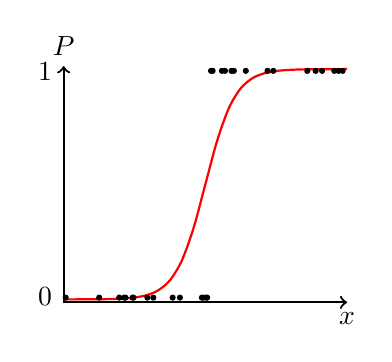
\begin{tikzpicture}[scale=0.15]
				% \draw [step=1, gray, very thin] (-12, -10) grid (12, 10);
				\draw [thick, <->] (-12, 10) node [anchor=south] {$P$} -- (-12, -10) -- (12, -10) node [anchor=north] {$x$};
				\draw [red, thick, smooth] plot [domain=-12:12] (\x, {(1 / (1 + exp(-0.8*\x)))*19.5 - 9.75});
				\draw plot [only marks, mark=*, mark size=6, domain=-8:8, samples=15] ({12.5*rnd - 0.5}, 9.6);
				\draw plot [only marks, mark=*, mark size=6, domain=-8:8, samples=15] ({-12.5*rnd + 0.5}, -9.6);
				\draw (-15, -9.5) node [anchor=west] {$0$};
				\draw (-15, 9.5) node [anchor=west] {$1$};
			\end{tikzpicture}
		\end{multicols}
		
		\columnbreak
		
		\section*{Statistical definitions}
		
		Let $\xi, \eta$ be random variables, $a, b \in \mathbb{R}$ constants, and $P$ denotes probability.
		
		\subsection*{Mean}
		
		Definition: \quad $E(\xi) = \sum_{i=1}^{n}\xi_{i} \cdot P[\xi = \xi_{i}]$
		
		\begin{multicols}{2}
			Population mean:
			
			\begin{center}
				$\E(\xi) = \dfrac{1}{N}\sum_{i=1}^{N}\xi_{i}$
			\end{center}
			
			\columnbreak
			
			Sample mean:
			
			\begin{center}
				$\E(\xi) = \dfrac{1}{n}\sum_{i=1}^{n}\xi_{i}$
			\end{center}
		\end{multicols}
		
		Some properties:
		
		\begin{itemize}[leftmargin=*]
			\item $\E(a) = a$
			\item $\E(\xi + a) = \E(\xi) + a$
			\item $\E(a \cdot \xi) = a \cdot \E(\xi)$
			\item $\E(\xi \pm \eta) = \E(\xi) + \E(\eta)$
			\item $\E(\xi \cdot \eta) = \E(\xi) \cdot \E(\eta)$ \quad only if $\xi$ and $\eta$ are independent.
			\item $\E(\xi - \E(\xi)) = 0$
			\item $\E(a \cdot \xi + b \cdot \eta) = a \cdot \E(\xi) + b \cdot \E(\eta)$
		\end{itemize}
		
		\subsection*{Variance}
		
		Definition: \quad $\Var(\xi) = \E[(\xi - \E(\xi))^{2}]$
		
		\begin{multicols}{2}
			Population variance:
			
			\begin{center}
				$\Var(\xi) = \dfrac{\sum_{i=1}^{N} (\xi_{i} - \E(\xi))^2}{N}$
			\end{center}
			
			\columnbreak
			
			Sample variance:
			
			\begin{center}
				$\Var(\xi) = \dfrac{\sum_{i=1}^{n} (\xi_{i} - \E(\xi))^2}{n - 1}$
			\end{center}
		\end{multicols}
		
		Some properties:
		
		\begin{itemize}[leftmargin=*]
			\item $\Var(a) = 0$
			\item $\Var(\xi + a) = \Var(\xi)$
			\item $\Var(a \cdot \xi) = a^{2} \cdot \Var(\xi)$
			\item $\Var(\xi \pm \eta) = \Var(\xi) + \Var(\eta) \pm 2 \cdot \Cov(\xi, \eta)$
			\item $\Var(a \cdot \xi \pm b \cdot \eta) = a^{2} \cdot \Var(\xi) + b^{2} \cdot \Var(\eta) \pm 2 a b \cdot \Cov(\xi, \eta)$
		\end{itemize}
		
		\subsection*{Covariance}
		
		Definition: \quad $\Cov(\xi, \eta) = \E[(\xi - E(\xi)) \cdot (\eta - E(\eta))]$
		
		\begin{multicols}{2}
			Population covariance:
			
			\begin{center}
				$\dfrac{\sum_{i=1}^{N} (\xi_{i} - \E(\xi)) \cdot (\eta_{i} - \E(\eta))}{N}$
			\end{center}
			
			\columnbreak
			
			Sample covariance:
			
			\begin{center}
				$\dfrac{\sum_{i=1}^{n} (\xi_{i} - \E(\xi)) \cdot (\eta_{i} - \E(\eta))}{n - 1}$
			\end{center}
		\end{multicols}
		
		Some properties:
		
		\begin{itemize}[leftmargin=*]
			\item $\Cov(\xi, a) = 0$
			\item $\Cov(\xi + a, \eta + b) = \Cov(\xi, \eta)$
			\item $\Cov(a \cdot \xi, b \cdot \eta) = a b \cdot \Cov(\xi, \eta)$
			\item $\Cov(\xi, \xi) = \Var(\xi)$
			\item $\Cov(\xi, \eta) = \Cov(\eta, \xi)$
		\end{itemize}
		
		\columnbreak
		
		\section*{Hypothesis testing}
		
		\begin{center}
			\begin{tabular}{ c | c | c }
				               & $H_{0}$ true            & $H_{0}$ false           \\ \hline
				Reject $H_{0}$ & False positive          & True positive           \\
				               & Type I Error $(\alpha)$ & $(1 - \beta)$           \\ \hline
				Accept $H_{0}$ & True negative           & False negative          \\
				               & $(1 - \alpha)$          & Type II Error $(\beta)$
			\end{tabular}
		\end{center}
		
		\columnbreak
		
		Typical one-tail test:
		
		\begin{center}
			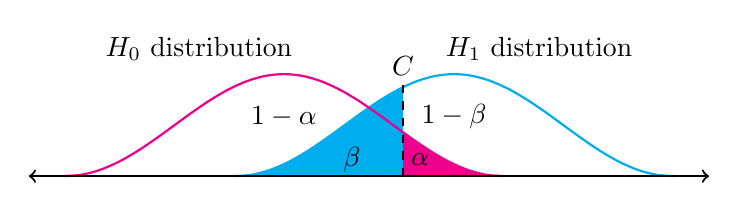
\begin{tikzpicture}[scale=0.108]
				\fill [magenta] (4, 0) -- plot [domain=4:16, smooth] (\x, {cos(\x*7 + 70)*6 + 6}); 
				\fill [cyan] (4, 0) -- plot [domain=-16:4, smooth] (\x, {cos(\x*7 - 70)*6 + 6}); 
				\draw [thick, cyan] plot [domain=-16:36, smooth] (\x, {cos(\x*7 - 70)*6 + 6}); 
				\draw [thick, magenta] plot [domain=-36:16, smooth] (\x, {cos(\x*7 + 70)*6 + 6}); 
				\draw [thick, <->] (-40, 0) -- (40, 0); 
				\draw [thick, dashed] (4, 0) -- (4, 11); 
				\node at (-20, 15) {$H_{0}$ distribution};
				\node at (20, 15) {$H_{1}$ distribution}; 
				\node at (-10, 7) {$1 - \alpha$}; 
				\node at (10, 7) {$1 - \beta$}; 
				\node at (6, 2) {$\alpha$}; 
				\node at (-2, 2) {$\beta$}; 
				\node at (4, 13) {$C$};
			\end{tikzpicture}
		\end{center}
		
		where $(1 - \alpha)$ is the confidence level, $\alpha$ is the significance level, $C$ is the critical value, $(1 - \beta)$ is the statistical power.
		
		\section*{Bootstraping}
		
		\textbf{Problem} - Asymptotic approximations to the distributions of test statistics do not work on small samples.
		
		\textbf{Solution} - Boostrap is basically sampling with replacement. The observed data is treated like a population, and multiple samples are exracted to recalculate an estimator or test statistic multiple times (improve accuracy).
	\end{multicols}
	
	\begin{multicols}{2}
		\section*{VAR (Vector Autoregressive)}
		
		A VAR model captures \textbf{dynamic interactions} between time series. The VAR($p$):
		
		\begin{center}
			$y_{t} = A_{1} y_{t - 1}+ \cdots + A_{p} y_{t - p} + B x_{t} + CD_{t} + u_{t}$
		\end{center}
		
		where:
		
		\begin{itemize}[leftmargin=*]
			\item $y_{t} = (y_{1t}, \ldots, y_{Kt})^{\tr}$ is a vector of $K$ observable endogenous time series.
			\item $A_{i}$'s are $K \times K$ coefficient matrices.
			\item $x_{t} = (x_{1t}, \ldots, x_{Mt})^{\tr}$ is a vector of $M$ observable exogenous time series.
			\item $B$ is an $K \times M$ coefficient matrix.
			\item $D_{t}$ is a vector that contains all deterministic terms: a constant, linear trend, seasonal dummy, and/or any other user specified dummy variables.
			\item $C$ is a coefficient matrix of suitable dimension.
			\item $u_{t} = (u_{1t}, \ldots, u_{Kt})^{\tr}$ is a vector of $K$ white noise series.
		\end{itemize}
		
		\textbf{Stability condition}:
		
		\begin{center}
			$\det(I_{K} - A_{1} z - \cdots - A_{p} z^{p}) \neq 0 \quad \mathrm{for}\quad \lvert z \rvert \leq 1$
		\end{center}
		
		\quad this is, there are \textbf{no roots} in and on the complex unit circle.
		
		For example, a VAR model with two endogenous variables ($K = 2$), two lags ($p = 2$), an exogenous contemporaneous variable ($M = 1$), a constant ($\mathrm{const}$) and a trend ($\mathrm{Trend}_{t}$):
		
		\begin{center}
			\scalebox{0.80}{
				$
				\begin{bmatrix}
					y_{1t} \\
					y_{2t}
				\end{bmatrix}
				=
				\begin{bmatrix}
					a_{11, 1} & a_{12, 1} \\
					a_{21, 1} & a_{22, 1}
				\end{bmatrix}
				\cdot
				\begin{bmatrix}
					y_{1, t - 1} \\
					y_{2, t - 1}
				\end{bmatrix}
				+
				\begin{bmatrix}
					a_{11, 2} & a_{12, 2} \\
					a_{21, 2} & a_{22, 2}
				\end{bmatrix}
				\cdot
				\begin{bmatrix}
					y_{1, t - 2} \\
					y_{2, t - 2}
				\end{bmatrix}
				+
				\begin{bmatrix}
					b_{11} \\
					b_{21}
				\end{bmatrix}
				\cdot
				\begin{bmatrix}
					x_{t}
				\end{bmatrix}
				+
				\begin{bmatrix}
					c_{11} & c_{12} \\
					c_{21} & c_{22}
				\end{bmatrix}
				\cdot
				\begin{bmatrix}
					\mathrm{const}     \\
					\mathrm{Trend}_{t}
				\end{bmatrix}
				+
				\begin{bmatrix}
					u_{1t} \\
					u_{2t}
				\end{bmatrix}
				$
			}
		\end{center}
		
		Visualizing the separate equations:
		
		\begin{center}
			$y_{1t} = a_{11, 1} y_{1, t - 1} + a_{12, 1} y_{2, t - 1} + a_{11, 2} y_{1, t - 2} + a_{12, 2} y_{2, t - 2} + b_{11} x_{t} + c_{11} + c_{12} \mathrm{Trend}_{t} + u_{1t}$
			
			$y_{2t} = a_{21, 1} y_{2, t - 1} + a_{22, 1} y_{1, t - 1} + a_{21, 2} y_{2, t - 2} + a_{22, 2} y_{1, t - 2} + b_{21} x_{t} + c_{21} + c_{22} \mathrm{Trend}_{t} + u_{2t}$
		\end{center}
		
		If there is an unit root, the determinant is zero for $z = 1$, then some or all variables are integrated and a VAR model is no longer appropiate (is unstable).
		
		\subsection*{SVAR (Structural VAR)}

		In a VAR model, causal interpretation is not explicit and results are sensitive to variable ordering. An SVAR extends VAR by imposing theory-based restrictions on $\mathsf{A}$ and/or $\mathsf{B}$ matrices. This can enable causal interpretation and shock analysis without reliance on arbitrary ordering.
		
		For example, a basic SVAR($p$) model:
		
		\begin{center}
			$\mathsf{A} y_t = \mathsf{A} [A_1, \ldots, A_p] y_{t - 1} + \mathsf{B} \varepsilon_t$
		\end{center}
		
		where:
		
		\begin{itemize}[leftmargin=*]
			\item $u_t = \mathsf{A}^{-1} \mathsf{B} \varepsilon_t$
			\item $\mathsf{A}$, $\mathsf{B}$ are ($K \times K$) matrices.
		\end{itemize}
		
		\columnbreak
		
		\section*{VECM (Vector Error Correction Model)}
		
		If \textbf{cointegrating relations} are present in a system of variables, the VAR form is not the most convenient. It is better to use a VECM, that is, the levels VAR substracting $y_{t - 1}$ from both sides. The VECM($p - 1$):
		
		\begin{center}
			$\Delta y_{t} = \Pi y_{t - 1} + \sum_{i = 1}^{p - 1} \Gamma_{i} \Delta y_{t - i} + B x_{t} + CD_{t} + u_{t}$
		\end{center}
		
		where:
		
		\begin{itemize}[leftmargin=*]
			\item $\Delta y_{t} = (\Delta y_{1t}, \ldots, \Delta y_{Kt})^{\tr}$ is a vector of $K$ observable endogenous time series.
			\item $\Pi y_{t - 1}$ is the \textbf{long-term} part.
			\begin{itemize}[leftmargin=*, label={$\diamond$}]
				\item $\Pi = - (I_{K} - A_{1} - \cdots - A_{p})$ for $i = 1, \ldots, p - 1$
				\item $\Pi = \alpha \beta^{\tr}$
				\item $\alpha$ is the \textbf{loading matrix} ($K \times r$). It represents the speed-of-adjustment.
				\item $\beta$ is the \textbf{cointegration matrix} ($K \times r$).
				\item $\beta^{\tr} y_{t - 1}$ is the \textbf{cointegrating equation}. It represents the long-run equilibrium.
				\item $\rk(\Pi) = \rk(\alpha) = \rk(\beta) = r$ is the \textbf{cointegrating rank}.
			\end{itemize}
			\item $\Gamma_{i} = - (A_{i + 1} + \cdots + A_{p})$ for $i = 1, \ldots, p - 1$ are the \textbf{short-term} parameters.
			\item $x_{t}$, $B$, $C$, $D_{t}$ and $u_{t}$ are as in VAR.
		\end{itemize}
		
		For example, a VECM with three endogenous variables ($K = 3$), two lags ($p = 2$) and two cointegratig relations ($r = 2$):
		
		\begin{center}
			$\Delta y_{t} = \Pi y_{t - 1} + \Gamma_{1} \Delta y_{t - 1} + u_{t}$
		\end{center}
		
		\quad where:
		
		\begin{center}
			\scalebox{0.95}{
				$\Pi y_{t - 1} = \alpha \beta^{\tr} y_{t - 1} =
				\begin{bmatrix}
					\alpha_{11} & \alpha_{12} \\
					\alpha_{21} & \alpha_{22} \\
					\alpha_{31} & \alpha_{32}
				\end{bmatrix}
				\begin{bmatrix}
					\beta_{11} & \beta_{21} & \beta_{31} \\
					\beta_{12} & \beta_{22} & \beta_{32}
				\end{bmatrix}
				\begin{bmatrix}
					y_{1, t - 1} \\
					y_{2, t - 1} \\
					y_{3, t - 1}
				\end{bmatrix}
				=
				\begin{bmatrix}
					\alpha_{11} ec_{1, t - 1} + \alpha_{12} ec_{2, t - 1} \\
					\alpha_{21} ec_{1, t - 1} + \alpha_{22} ec_{2, t - 1} \\
					\alpha_{31} ec_{1, t - 1} + \alpha_{32} ec_{2, t - 1}
				\end{bmatrix}
				$
			}
		\end{center}
		
		\vspace*{0.2cm}
		
		\begin{center}
			$ec_{1, t - 1} = \beta_{11} y_{1, t - 1} + \beta_{21} y_{2, t - 1} + \beta_{31} y_{3, t - 1}$
			
			$ec_{2, t - 1} = \beta_{12} y_{1, t - 1} + \beta_{22} y_{2, t - 1} + \beta_{32} y_{3, t - 1}$
		\end{center}
		
		\quad and
		
		\begin{center}
			\scalebox{0.95}{
				$\Gamma_{1} \Delta y_{t - 1} = 
				\begin{bmatrix}
					\gamma_{11} & \gamma_{12} & \gamma_{13} \\
					\gamma_{21} & \gamma_{22} & \gamma_{23} \\
					\gamma_{31} & \gamma_{32} & \gamma_{33}
				\end{bmatrix}
				\begin{bmatrix}
					\Delta y_{1, t - 1} \\
					\Delta y_{2, t - 1} \\
					\Delta y_{3, t - 1}
				\end{bmatrix}
				\quad
				u_t =
				\begin{bmatrix}
					u_{1} \\
					u_{2} \\
					u_{3}
				\end{bmatrix}
				$
			}
		\end{center}
		
		Visualizing the separate equations:
		
		\begin{center}
			$\Delta y_{1t} = \alpha_{11} ec_{1, t - 1} + \alpha_{12} ec_{2, t - 1}  + \gamma_{11} \Delta y_{1, t - 1} + \gamma_{12} \Delta y_{2, t - 1} + \gamma_{13} \Delta y_{3, t - 1} + u_{1t}$
			
			$\Delta y_{2t} = \alpha_{21} ec_{1, t - 1} + \alpha_{22} ec_{2, t - 1}  + \gamma_{21} \Delta y_{1, t - 1} + \gamma_{22} \Delta y_{2, t - 1} + \gamma_{23} \Delta y_{3, t - 1} + u_{2t}$
			
			$\Delta y_{3t} = \alpha_{31} ec_{1, t - 1} + \alpha_{32} ec_{2, t - 1}  + \gamma_{31} \Delta y_{1, t - 1} + \gamma_{32} \Delta y_{2, t - 1} + \gamma_{33} \Delta y_{3, t - 1} + u_{3t}$
		\end{center}
	\end{multicols}
\end{document}